% Please do not change the document class
\documentclass{scrartcl}

% Please do not change these packages
\usepackage[hidelinks]{hyperref}
\usepackage[none]{hyphenat}
\usepackage{setspace}
\usepackage{listings}
\doublespace

% You may add additional packages here
\usepackage{amsmath}
\usepackage{graphicx} 
\graphicspath{ {Diagrams/} }

% Please include a clear, concise, and descriptive title
\title{COMP210 - VR Interface Design Document}

% Please put your student number in the author field
\author{1507866}

\begin{document}
	
\maketitle
The interface I've designed uses the HTC Vive and controllers. Due to time constraints and lack of parts I couldn't set up the Arduino however I have integrated the code into Unity and written the Arduino code so it is ready to be used and just requires the Arduino and servos to be plugged in. 

\begin{figure}[h]
	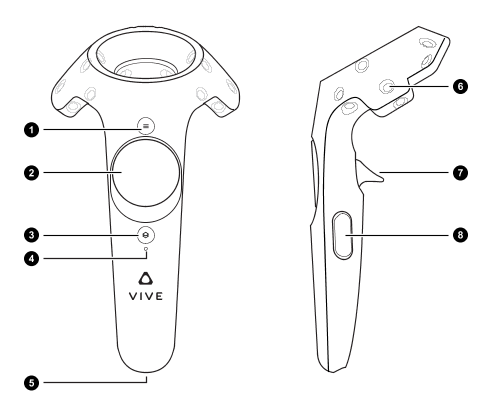
\includegraphics[width=0.8\linewidth]{vive_controller.png}
	\caption{Vive Controllers  }
\end{figure} 

The player uses the Vive HMD and controllers to interact with the interface. The HMD moves the camera and the controllers are used to interact with the bird.  The player presses the trigger on the right controller to summon the falcon which will move towards the controller. When the game registers a collision between the controller and the falcon it sends out a ``p" through the serial which can be received by an Arduino. This uses the SerialCommUnity package for Unity to send characters through the serial.

\begin{figure}[h]
	\includegraphics[width=1.0\linewidth]{unity_code.png}
	\caption{ Unity code for communicating with Arduino }
\end{figure} 

Above shows the C\# code used to send the character through the serial.

On receiving the serial input the Arduino moves the servos to specified position using the code below.

\section{Arduino Code}
\begin{lstlisting}
#include <Servo.h>
Servo clawServos[2];  
// creates and arrary of servos 
int pos = 0; 
String inputString = "";
boolean stringComplete = false;

void setup() {
	Serial.begin(9600);
	inputString.reserve(200);
	clawServos[0].attach(9);
	clawServos[1].attach(10);
	// attaches the servos on pin 9 and 10 to the servo object   
}
void loop() {
	if (stringComplete) {
	Serial.println(inputString);
	inputString = " ";
	stringComplete = false;
	}
}

void serialEvent() {
	while(Serial.available()) {
	char inChar = (char)Serial.read();
	inputString += inChar;
	
	if (inChar == '\n') {
		stringComplete = true;
	}
	
	if (inChar == 'p'){
		pinch();
		}
	}
}
void pinch() {
	for (pos = 0; pos <= 180; pos += 1) {
	// goes from 0 degrees to 180 degrees
	// in steps of 1 degree
	for (i = 0; i <= sizeof(clawServos); i += 1) {
			clawServos[i].write(pos);  
			// tell servo to go to position in variable 'pos'
	}
      
	delay(15);                       
	// waits 15ms for the servo to reach the position
	}
	for (pos = 180; pos >= 0; pos -= 1) { 
		// goes from 180 degrees to 0 degrees
		for (i = 0; i <= sizeof(clawServos); i += 1) {
			clawServos[i].write(pos); 
		}
		delay(15);
	}
}

\end{lstlisting}

Both servos move at the same time to simulate falcon claws as the falcon lands on the players arm in game.

\newpage
\section{Arduino Diagram}

\begin{figure}[h]
	\includegraphics[width=1.0\linewidth]{arduino_diagram.png}
	\caption{ Arduino Uno and two servos }
\end{figure} 
The diagram above shows how the servos and Arduino would be connected. I would also want to add a wireless connection between the Arduino and computer running the game as VR already involves many wires so it would be easier for the player to have the Arduino wireless on their arm. 

\bigskip



\bibliographystyle{ieeetr}
	
\end{document}
